\begin{alertblock}{What is the model looking at?}
Using the feature analysis tool Shap \cite{lundberg2017unified}, we find that:
\begin{itemize}
  \item Not only low redshifts measurements are relevant for predictions based on growth rate.
  \item The models values the $P(k)$ derivatives at quasi non-linear and non-linear scales over the peak position
\end{itemize}.
\vspace{-2ex}
 \begin{figure}[h]
   \centering
   \begin{subfigure}{0.48\textwidth}
     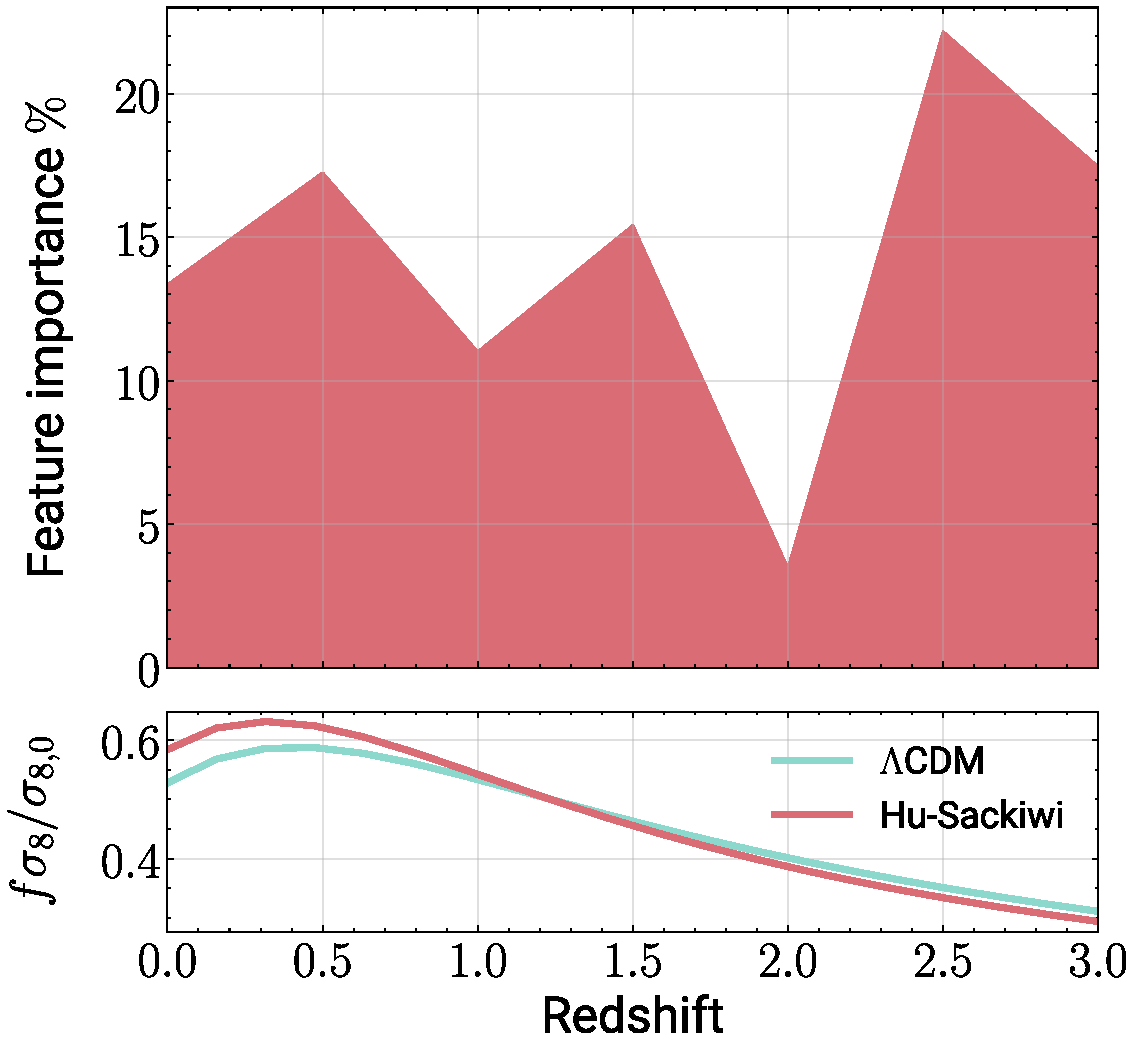
\includegraphics[width=\textwidth]{figures/fs8_features.pdf}
     
   \end{subfigure}\hfill
   \begin{subfigure}{0.477\textwidth}
     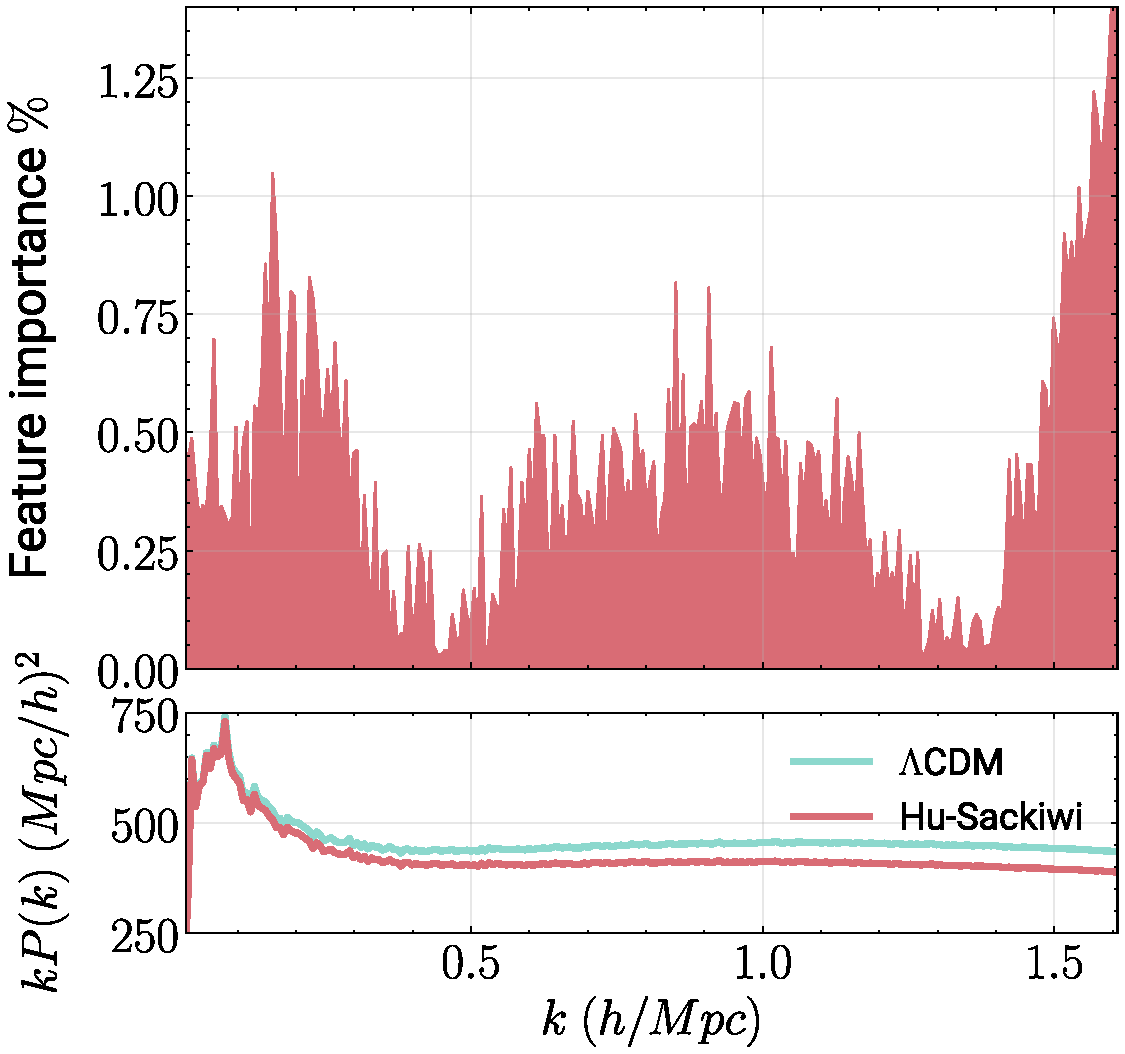
\includegraphics[width=\textwidth]{figures/pk_features.pdf}

   \end{subfigure}
   \caption{Feature analysis compared to MGCAMB results for reference.}
 \end{figure}

\end{alertblock}